\setchapterpreamble[u]{\margintoc\hfil}
\chapter{Results}
\labch{results}

The following sections look at the built spectrometer from a user's point of view. The first \refsec{user-perspective} describes the assembly and operation of the spectrometer built above. The following \refsec{water-signal} discusses how to measure a signal with water as a simple and approachable example.

\section{The spectrometer from a user's perspective}
\labsec{user-perspective}
The spectrometer was designed with ease of use and reconfigurability in mind. The individual parts are placed on separate boards, connected with standard \acrshort{sma} connectors. Broken parts can thus be easily exchanged. Old already existing parts can be used in conjunction with newly developed ones, facilitating the re-use of hardware and ensuring operation while a broken part is fixed or upgraded.

The software -- while still incomplete -- has the same goals as the hardware. It's written in \gls{python} with extensive documentation, comments throughout the code and accompanying guides to get started\sidenote{Take a look at the official \lstinline{README.md} in the \href{https://gitlab.ethz.ch/mstabel/nmr-spectrometer/-/tree/master/software/spectrometer}{official repository}}. Generally, the code tries to adhere to the ideas presented in \enquote{Uncle Bob's} book \textit{Clean Code} \sidecite{martinCleanCodeHandbook2008}.

\begin{marginfigure}
    \includesvg{images/logo_magnETHical.svg}
    \caption{Logo of the \textit{magnETHical} spectrometer project}
    \labfig{logo-magnethical}
\end{marginfigure}

There are five main parts to the spectrometer as explained in \nrefch{concepts}:
\begin{description}
    \item[The console] (i.e. the RedPitaya) responsible for sending, receiving and processing the \acrshort{rf} signals.
    \item[The power amplifiers] responsible for amplifying the signal generated by the console
    \item[The transmit-receive switch] responsible for switching between sending a signal into the probe from the transmit channel and receiving a signal back from the probe into the receive channel
    \item[The probe] consisting of the probe holder and the probe coil, responsible for emitting and receiving the \acrshort{rf} signal
    \item[The \acrlong{lna}s] responsible for amplifying the weak signal received by the probe before feeding it to the console for processing
\end{description}
The short conceptual overview is reproduced in figure \reffig{overview} for the reader's convenience. Each output needs to be connected to the input of the next device. The power connections are not shown in favour of clarity, but each part is labelled with the possible input voltages, in a range of \qtyrange{7}{15}{\volt}. For a more detailed description of the individual parts and their connections see the \enquote{magnETHical} project page (compare \reffig{logo-magnethical}) or the descriptions above.

\begin{figure*}[!htb]
    \centering
    \begin{circuitikz}[european]
        \ctikzset{bipoles/amp/width=0.9}
        \draw[nodes={align=center}]
        (0,0) coordinate(mid)

        % RP
        (mid) node[draw, align=center, minimum height=5.5cm, minimum width=2cm](redpitaya){Red\\Pitaya\\SDRlab\\122-16}
        ($(redpitaya.east)!0.75!(redpitaya.north east)$) coordinate(rptx) node[left]{TX\\(Out 1)}
        ($(redpitaya.east)!0.75!(redpitaya.south east)$) coordinate(rprx) node[left]{RX\\(In 1)}

        % TX
        (rptx) to[lowpass,l=SCLF-27+,>] ++(5,0)
        to[amp,t=\acrshort{pa},l=ADL5536\\PHA-202+,>] ++(5,0) coordinate(tx)

        % Circulator
        (mid -| tx) node[circulator,label={left:QPC6324}](circ){}
        (tx) -| (circ.n) node[inputarrow,rotate=270]{}

        % RX
        (rprx -| circ) coordinate(rx)
        (circ.s) |- (rx)
        (rx) to[amp,t=\acrshort{lna},l=PHA-13LN+,>] ++(-2.5,0)
        to[amp,t=\acrshort{lna},l=PHA-13LN+,>] ++(-2.5,0)
        to[amp,t=\acrshort{lna},l=PHA-13LN+,>] ++(-2.5,0)
        to[lowpass,l=SCLF-27+,>] ++(-2.5,0) node[inputarrow,rotate=180]{}

        % Probe
        (circ.e) -- ++(1,0)
        node[dinantenna](probe){}
        node[below=1ex]{3D-printed\\probe holder}
        ;
    \end{circuitikz}

    \caption{\captiontitle{Component overview.} The schematic contains all physical parts of the \acrshort{nmr} spectrometer that need to be connected through \acrshort{sma} cables.}
    \labfig{overview}
\end{figure*}

Having ordered or built the parts, connected them using \acrshort{sma} cables and powered them through a lab power supply, the console needs to be configured. The configuration of the console is relatively simple as most of the complexity has been programmed into the \gls{python} control library. The user thus only needs to ensure that a working \acrshort{linux} distribution is running on the \acrshort{rp} and that the \acrshort{ip} address is known. The official distribution that is pre-installed on the micro SD card that ships with the \acrshort{rp} is completely sufficient.

If the user needs to create a new microSD card, the \url{setup of the microSD card is described in the \acrshort{rp} docs}{https://redpitaya.readthedocs.io/en/latest/quickStart/SDcard/SDcard.html} and is summarized here for simplicity on a Linux based system.

\begin{enumerate}
    \item \url{Download the newest release}{https://redpitaya.readthedocs.io/en/latest/quickStart/SDcard/SDcard.html}
    \item Insert the microSD card into your computer.
    \item Figure out its name using \lstinline{lsblk} or \lstinline{df -h}, e.g. \lstinline{/dev/mmcblk0} or \lstinline{/dev/sdc}.
    \item
    \item
\end{enumerate}


\todo{Wassersignal Spannung (aus vergleich mit Funktionsgeneratorsignal)}

\section{Measuring a water signal}
\labsec{water-signal}
\begin{marginfigure}
    \centering
    \includesvg{simple_pulse_sequence.svg}
    \caption{\captiontitle{Simple pulse sequence} The usual depiction of a simple pulse sequence. The \enquote{RF pulse} is a high frequency \acrshort{rf} pulse close to the resonance frequency of the nuclei to be observed. After the pulse, a decaying sinus signal can be received on the same coil -  the so-called \acrfull{fid}.}
    \labfig{simple-pulse-sequence}
\end{marginfigure}

\begin{figure}[h!bt]
    \centering
    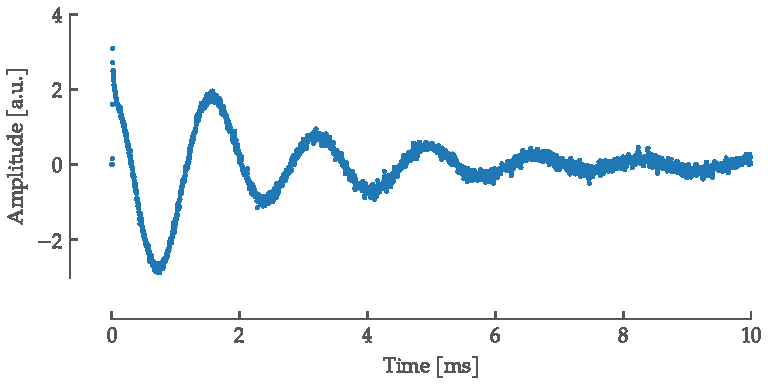
\includegraphics{fid_raw.pdf}
    \caption{\captiontitle{\acrfull{fid} of water.} The signal was recorded after a \qty{9}{\micro\second} impulse of a strength of \qty{1}{\watt} and a delay of \qty{25}{\micro\second}, waiting for the coil to ring down. \enquote{Andrew's probe} was used in this measurement}
    \labfig{fid-raw}
\end{figure}

\begin{figure}[h!bt]
    \centering
    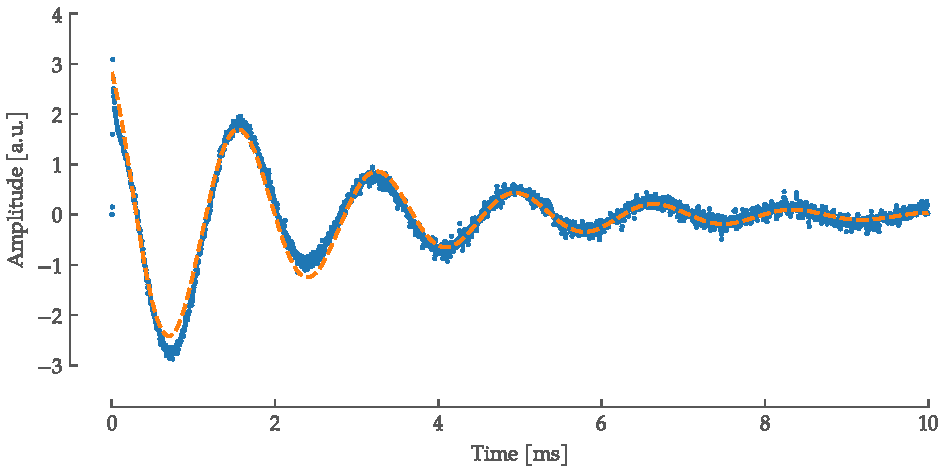
\includegraphics{fid_sine_fit.pdf}
    \caption{\captiontitle{\acrfull{fid} of water with a sine fit.} The blue data is the same as in \reffig{fid-raw}. The orange dashed line is the result of a least squares fit of a decaying sinus. It shows an exponential decay in amplitude with a $T_2^*$ of \qty{2.5}{ms} and a dominant frequency of about \qty{590}{\hertz}}
    \labfig{fid-sine-fit}
\end{figure}

\begin{figure}[h!bt]
    \centering
    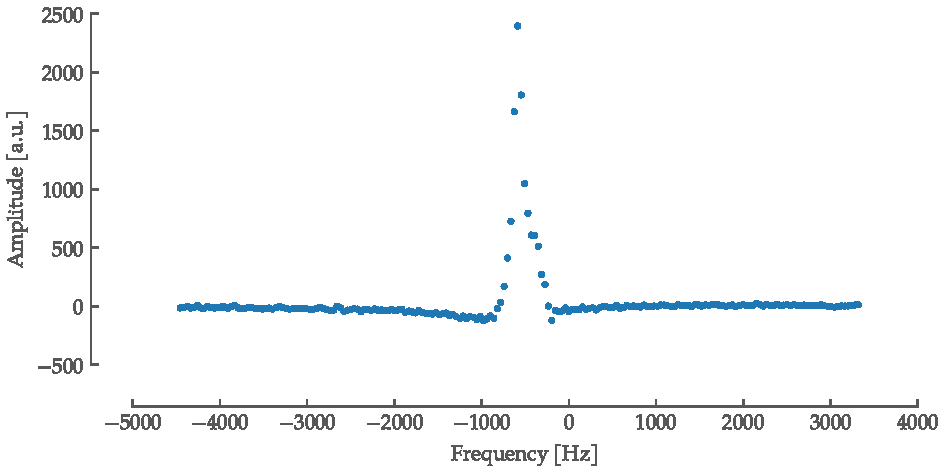
\includegraphics{fft_raw.pdf}
    \caption{\captiontitle{Fourier spectrum of \reffig{fid-raw}.} It shows a Lorentz-shaped peak around roughly \qty{600}{\hertz} with a slight broadening on the right side. The data was obtained through an automatic zero fill, complex Fouriertransform and an automated zero order phase correction of \ang{37}.}
    \labfig{fft-raw}
\end{figure}

\begin{figure}[h!bt]
    \centering
    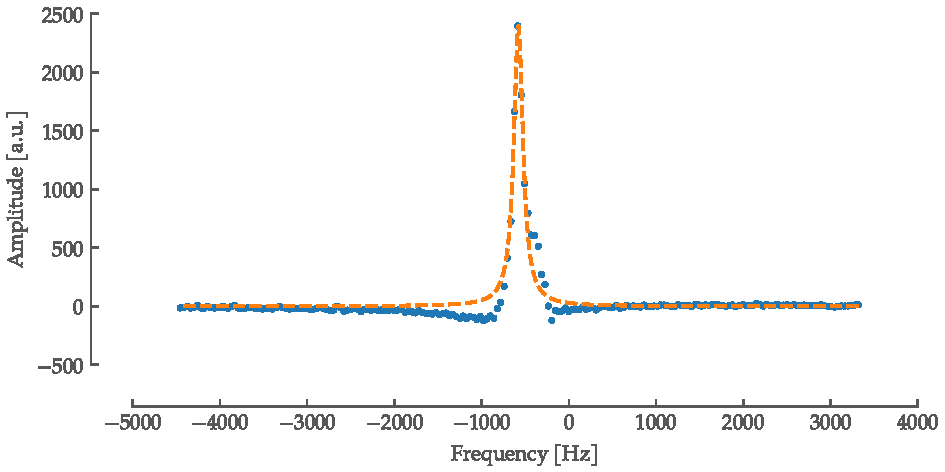
\includegraphics{fft_fit.pdf}
    \caption{\captiontitle{Fourier spectrum of \reffig{fid-raw} with lorentzian fit.} The Lorentzian curve was fit using a least-squares minimization approach. It's centred around \qty{-576}{\hertz} with a full width at half maximum of \qty{158}{\hertz}.}
    \labfig{fft-fit}
\end{figure}



\begin{figure}[h!bt]
    \centering
    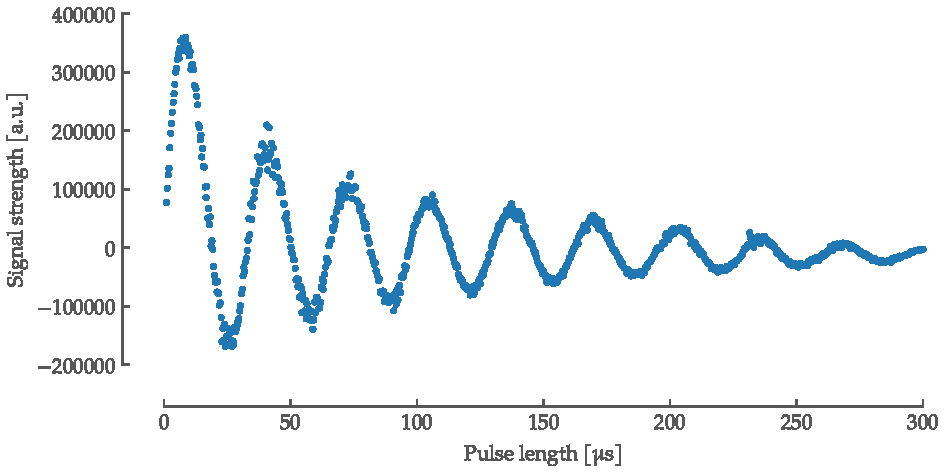
\includegraphics{rabi_nutation_raw.pdf}
    \caption{\captiontitle{Rabi nutation of the water signal}. Each data point was generated by performing an \acrshort{fid} experiment as described in \reffig{fid-raw} and integrating over the resulting peak (see \reffig{fft-raw}) to obtain a measure of signal strength. The phase correction applied to all points was identical.}
    \labfig{fft-fit}
\end{figure}

\begin{figure}[h!bt]
    \centering
    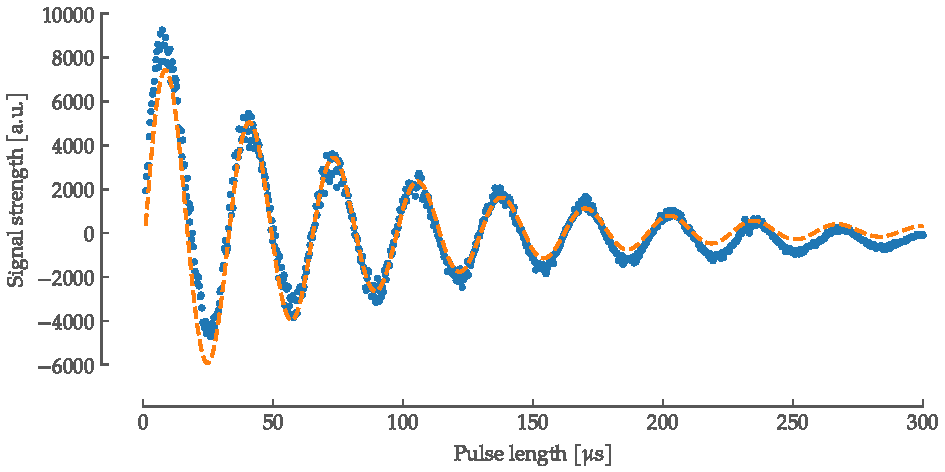
\includegraphics{rabi_nutation_fit.pdf}
    \caption{\captiontitle{Rabi nutation of the water signal with decaying sinus fit}. The data was fit using a least-squares approach to fit a decaying sinusoidal function. The fit has a period of \qty{32}{\micro\second}, giving the length of a $\frac{\pi}{2}$-pulse of \qty{8}{\micro\second}.}
    \labfig{fft-fit}
\end{figure}

\begin{marginfigure}
    \centering
    \includesvg{spin_echo_sequence_margin.svg}
    \caption{\captiontitle{Spin echo sequence}. A possible depiction of the spin echo sequence. A pulse of a duration that causes a \(\frac{\pi}{2}\) rotation of the spins and a pulse twice as long (i.e. length \(\pi\)) are applied with a delay of duration \(\tau\) in between. A spin echo is then observed with its peak after a delay of \(\tau\) after the second pulse.}
    \labfig{pulse-echo-sequence}
\end{marginfigure}

\begin{figure}[h!bt]
    \centering
    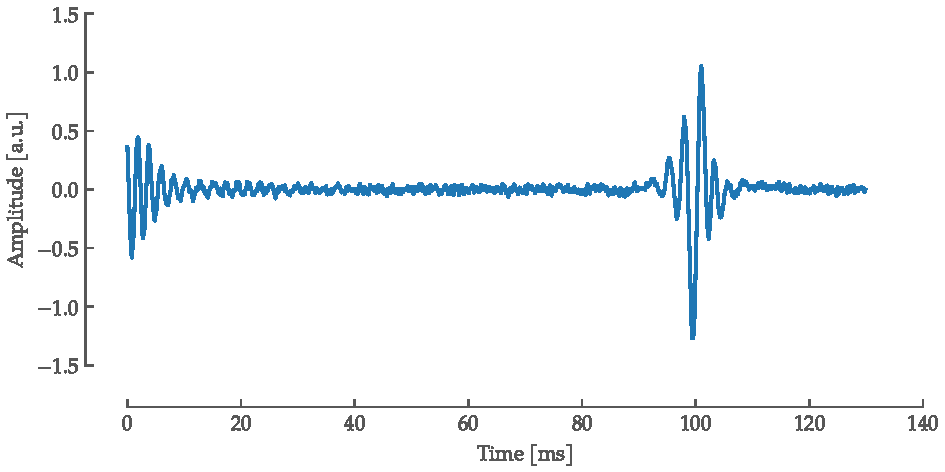
\includegraphics{spin_echo_avg.pdf}
    \caption{\captiontitle{Spin Echo}. Measurement of the received signal after the last pulse of a classic spin echo sequence (see \reffig{pulse-echo-sequence}). The \(\frac{\pi}{2}\) of \qty{9}{\micro\second} was sent with a power of \qty{1}{\watt}. The delay between pulses \(\tau\) was \qty{100}{\milli\second}. Data was recorded for \qty{130}{\milli\second} after the last pulse.}
    \labfig{spin-echo}
\end{figure}

\begin{marginfigure}
    \centering
    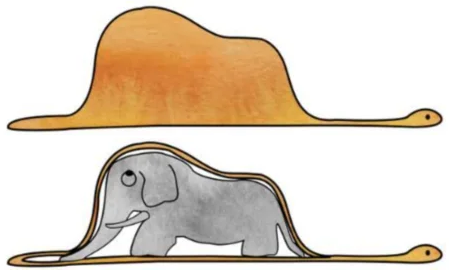
\includegraphics{little_prince_hat.png}
    \caption{\captiontitle{Le Petit Prince}. \enquote{My drawing was not a picture of a hat. It was a picture of a boa constrictor digesting an elephant.}\\
        --- Antoine de Saint-Exupéry}
    \labfig{pulse-echo-sequence}
\end{marginfigure}

\begin{figure}[h!bt]
    \centering
    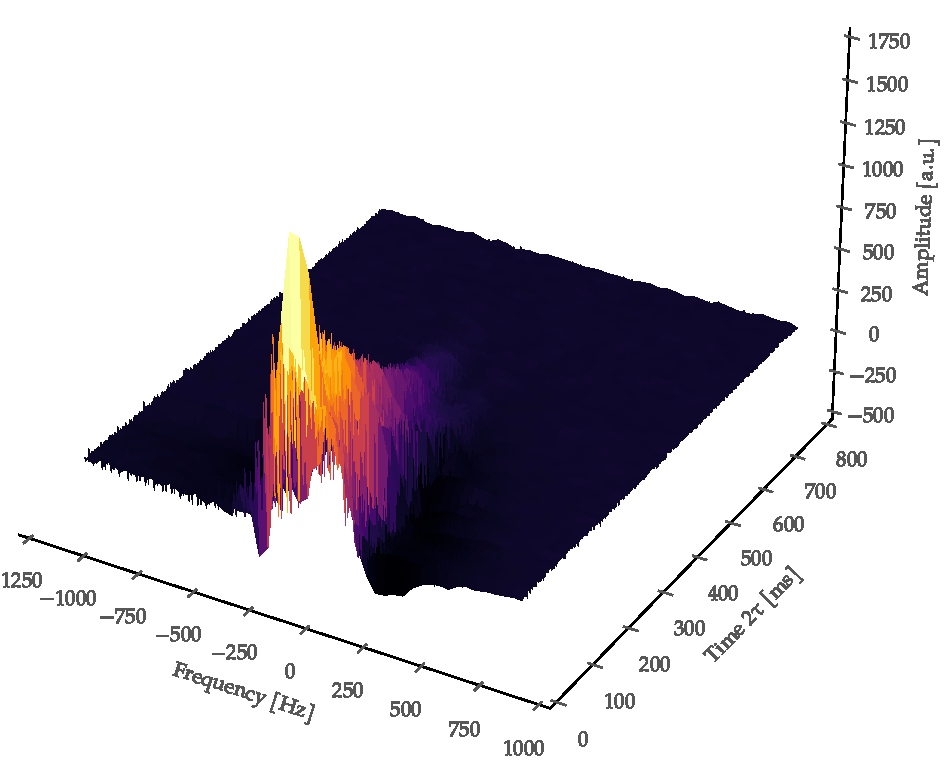
\includegraphics{t2_decay_3d_fft.pdf}
    \caption{\captiontitle{Fourier Transform of decaying spin echoes over delay length \(\tau\)}. The phase-corrected Fourier transforms are plotted in three dimensions over the delay \(\tau\) in between the pulses. The decay of the signal strength with increasing delay is clearly visible.}
    \labfig{t2-decay-3d}
\end{figure}

\begin{figure}[h!bt]
    \centering
    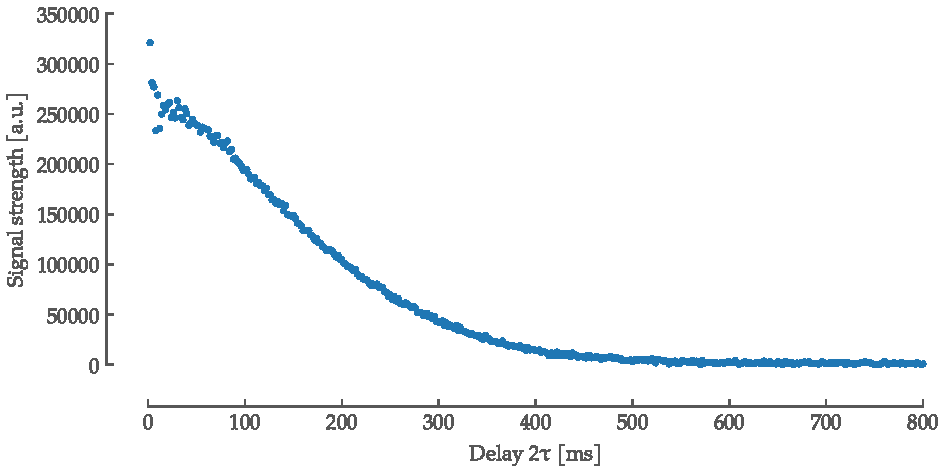
\includegraphics{t2_decay.pdf}
    \caption{\captiontitle{\(T_2\) decay of water}. Each data point is obtained by integrating the peak of the phase-corrected Fourier spectrum of a spin echo experiment as seen in \reffig{t2-decay-3d}. One can vaguely discern the expected exponential decay.}
    \labfig{t2-decay}
\end{figure}

\begin{figure}[h!bt]
    \centering
    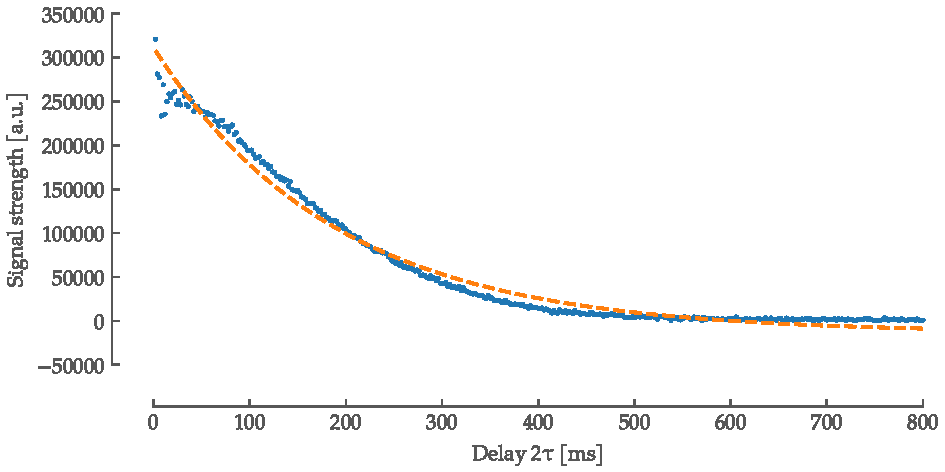
\includegraphics{t2_decay_fit.pdf}
    \caption{\captiontitle{\(T_2\) decay of water with an exponentially decaying function fitted}. The data points are the same as in \reffig{t2-decay}. The least-squares fit has a \(T_2\) decay time of \qty{190}{\milli\second}.}
    \labfig{t2-decay-fit}
\end{figure}

\section{Measuring a Toluol signal}
\labsec{toluol-signal}
\todo{Try and measure a Toluol (?) signal}